\chapter{Experimental Simulation and Analysis}
\label{chapter:Experimental Design and Analysis}

\section{Introduction}

The primary goal of this chapter is to demonstrate the application of the Particle Filter-Based Signalized Intersection Queue Estimator (PF-SIQE) developed in this thesis, focusing on validating the core aspects of the model through simulation experiments. These experiments aim to qualitatively evaluate the effectiveness of the PF-SIQE in tracking vehicle behavior and estimating states at signalized intersections, despite the inherent state and measurement uncertainties present in traffic systems.

Accurate queue length estimation is critical for optimizing traffic signal performance and improving traffic flow in intelligent transportation systems. Although the equations for computing queue lengths were introduced in Chapter 3, due to time constraints, this chapter will not present the queue length estimations. Instead, the focus will be on demonstrating the ground truth vehicle trajectories generated by the model. These trajectories will serve as a substitute for illustrating the system's ability to track vehicle behavior under various conditions.

Traditional approaches often struggle with the non-linearities and uncertainties typical of traffic behavior. The particle filter framework, with its capacity to manage non-linear and non-Gaussian processes, offers a promising solution for tackling these challenges. This chapter seeks to evaluate the proposed PF-SIQE model’s ability to track vehicle positions and predict their trajectories in response to dynamic traffic signal changes.

Given the limitations in coding, debugging, and time, this chapter focuses on validating specific components of the model, particularly the traffic decision-making model and the generation of ground truth measurements. While the full particle filter process, including its visualization, could not be fully executed, the groundwork for future implementation is established here.

The key objectives of the simulation experiments are as follows:
\begin{itemize}
    \item \textbf{Qualitative validation of the PF-SIQE:} The experiments aim to demonstrate that the filter can track vehicle behavior even when their decision-making process is influenced by stochastic factors, such as the dilemma zone, where vehicles must decide whether to stop or proceed. By providing inputs of traffic signals and simulated sensor measurements, the model is expected to qualitatively capture vehicle positions and ground truth trajectories in various traffic scenarios.
    \item \textbf{Analysis of simulation results:} The validation of the PF-SIQE will focus on analyzing the simulation results, comparing the model's output against the ground truth data generated in the simulation. This analysis will provide insights into how effectively the particle filter tracks vehicle behavior and whether the decision-making model functions as expected in different traffic scenarios.
    \item \textbf{Sensitivity analysis:} Various scenarios will be investigated to analyze the sensitivity of the model to different factors, such as detector placement, noise parameters, and the penetration rate of vehicles equipped with floating sensors.
\end{itemize}

The structure of this chapter is as follows: first, an overview of the simulation setup is provided, followed by a discussion of the validation results for the decision-making model and the analysis of ground truth trajectories. The chapter concludes with a sensitivity analysis list as future work, highlighting key factors influencing the performance of the PF-SIQE and suggestions for further development and testing.











\section{Experimental Setup}
This section describes the setup for the simulation experiments designed to validate the proposed estimator PF-SIQE. The focus is on the simulation environment, variables and parameters, models, and algorithms used.

\subsection{Simulation Environment}
To perform the simulation experiments, both software and hardware resources were utilized to ensure the accuracy and efficiency of the simulations.

\subsubsection{Software}
The simulations were conducted using MATLAB R2023b, which provides robust toolboxes for modeling, simulation, and implementation of particle filter algorithms. In this study, the Aerospace Toolbox 4.3, Control System Toolbox 10.12, and Statistics and Machine Learning Toolbox 12.4 were extensively used to model the traffic flow and implement the PF-SIQE. These toolboxes provided the necessary functions for handling state transitions, statistical analysis, and algorithmic implementations within the particle filter framework.


\subsubsection{Hardware 1}
The hardware 1 setup includes a computing environment with the following specifications:
\begin{itemize}
\item Processor: 2.3 GHz Quad-Core Intel Core i5
\item RAM: 8 GB 2133 MHz LPDDR3
\item Graphics: Intel Iris Plus Graphics 655 1536 MB
\item Operating System: macOS Monterey Version 12.6.6
\end{itemize}

\subsubsection{Hardware 2}
The hardware 2 setup includes a high-performance computing environment with the following specifications:
\begin{itemize}
\item Processor: 12th Gen Intel(R) Core(TM) i7-12700KF, 3.61 GHz
\item RAM: 32 GB
\item Graphics: unknown
\item Operating System: Microsoft Windows 11 Education, Version 10.0.22631
\end{itemize}

This setup ensures that the computationally intensive simulations, particularly those involving large numbers of particles and vehicles, run efficiently. The two hardware setups serve different purposes: the laptop (Hardware 1) is primarily used for running simulations during meetings and remote work, while the desktop (Hardware 2), with its higher processing power, is used for faster simulations and most of the code development at home. A Git-based workflow was employed to synchronize the codebase between the two machines, with code developed on the desktop pushed to a GitHub repository and then pulled onto the laptop when needed.


\subsection{Simulation Parameters}
For the sake of reproducibility, the simulation parameters used in the experiments are listed as follows. The parameters are categorized into two parts: those derived from the IDM model and literature, and tunable parameters specifically used for studying the sensitivity test.

\subsubsection{Parameters in longitudinal motion}
\begin{table}[htbp]
\small
    \centering
    \begin{tabular}{ccccccc}
    \toprule
         & desired  & maximum   & comfortable   & minimum   & safe time &  free flow  \\
         IDM & speed  &  acceleration  &  deceleration  &  gap  &  headway & exponent \\
         & \(v_{\text{desired}}\) (m/s) & $a_{\text{max}}$ (m/s$^2$)& $b$ (m/s$^2$) & $s_0$ (m) & $h_s$ (s) & \(\delta\)\\
        \hline
         value & 15.0 & 1.0 & 1.5 & 2.0 & 1.0& 4.0 \\
         \toprule
            & decision making & stop line   & reaction   &  deceleration   & yellow   & comfortable   \\
        TSDM &  boundary & position  &  time  &   rate  &  time  &  acceleration  \\
         & $D_h$ (m) & $d_\text{stop line}$ (m)& $T_{\text{reaction}}$ (s)& $b$ (m/s$^2$) & $T_{\text{yellow}}$ (s) & $a'$ (m/s$^2$) \\
        \hline
         value & 150 & 300 & 1.0 & 1.5 & 3.5 & 1.0 \\
         \toprule
    \end{tabular}
    \caption{The parameters in longitudinal motion (\textcite{treiber2013traffic}, \textcite{gates2007analysis})}
    \label{parameters in longitudinal motion}
\end{table}

\subsubsection{Tunable parameters}
\begin{table}[htbp]
    \centering
    \begin{tabular}{|l|l|}
        \hline
        \textbf{Parameter} & \textbf{Value} \\ \hline
        Time step ($\Delta t$) & 0.5 s \\ \hline
        Number of iterations & 60 \\ \hline
        Number of vehicles & 1 \\ \hline
        Number of particles & 5 \\ \hline
        Red light duration & 8 s \\ \hline
        Yellow light duration & 3.5 s \\ \hline
        Green light duration & 5 s \\ \hline
        Stop line position & 300 m \\ \hline
        Lane & 1 \\ \hline
        Decision distance ($D_h$) & 150 m \\ \hline
        Reaction time ($T_{\text{reaction}}$) & 1.0 s \\ \hline
        Probability of stopping in dilemma zone ($P_{\text{stop}}$) & 0.5 \\ \hline
        Maximum deceleration ($b_{\text{max}}$) & 1.5 m/s\(^2\) \\ \hline
        Initial position ($d_0$) & 50 m \\ \hline
        Discrete time step for traffic light decision ($T_{\text{discrete}}$) & 1 s \\ \hline
        Acceleration ($a$) & 1.0 m/s\(^2\) \\ \hline
        Stop decision & 1 \\ \hline
        Go decision & 2 \\ \hline
        Undecided decision & 3 \\ \hline
        Desired speed ($v_{\text{desired}}$) & 15 m/s \\ \hline
        Maximum acceleration ($a_{\text{max}}$) & 1.0 m/s\(^2\) \\ \hline
        Comfortable deceleration ($b$) & 1.5 m/s\(^2\) \\ \hline
        Minimum gap ($s_0$) & 2.0 m \\ \hline
        Vehicle length & 5.0 m \\ \hline
        Safe time headway ($T$) & 1.0 s \\ \hline
        Acceleration exponent ($\delta$) & 4 \\ \hline
        Acceleration noise ($n_a$) & 0.01 m/s\(^2\) \\ \hline
        Loop detector 1 position ($d_{\text{loop1}}$) & 150 m \\ \hline
        Loop detector 2 position ($d_{\text{loop2}}$) & 200 m \\ \hline
        Loop detector 3 position ($d_{\text{loop3}}$) & 250 m \\ \hline
        Time step for loop detector 1 & 1 s \\ \hline
        Time step for loop detector 2 & 1 s \\ \hline
        Time step for loop detector 3 & 1 s \\ \hline
        Accuracy of loop detector 2 & 0.95 \\ \hline
        GPS noise standard deviation ($\sigma_{\text{GPS}}$) & 5 m \\ \hline
        Effective sample size threshold (ESS) & 0.7 \\ \hline
    \end{tabular}
    \caption{Simulation parameters used in the experiments}
    \label{tab:simulation_parameters}
\end{table}










\section{Simulation}\label{Experimental Scenarios}
This section presents the simulation of ground truth states and measurements to validate the traffic decision-making model. It also outlines a list of scenarios for future experimentation, aimed at providing a comprehensive analysis of the PF-SIQE's capabilities, limitations, and areas for improvement. While these scenarios would offer valuable insights into the practical implementation and optimization of the estimator in real-world traffic management systems, due to time constraints, they will not be executed within this thesis.

\subsection{Ground Truth}

In this thesis, due to the lack of real data, the ground truth is simulated. The simulated ground truth consists of both state ground truth and measurement ground truth, generated by the state transition function and measurement function. By inputting the traffic signal, initial states, and corresponding noise distribution, the outputs produced are the ground truth, representing the actual states and actual measurements.

\begin{figure}[H]
    \centering
    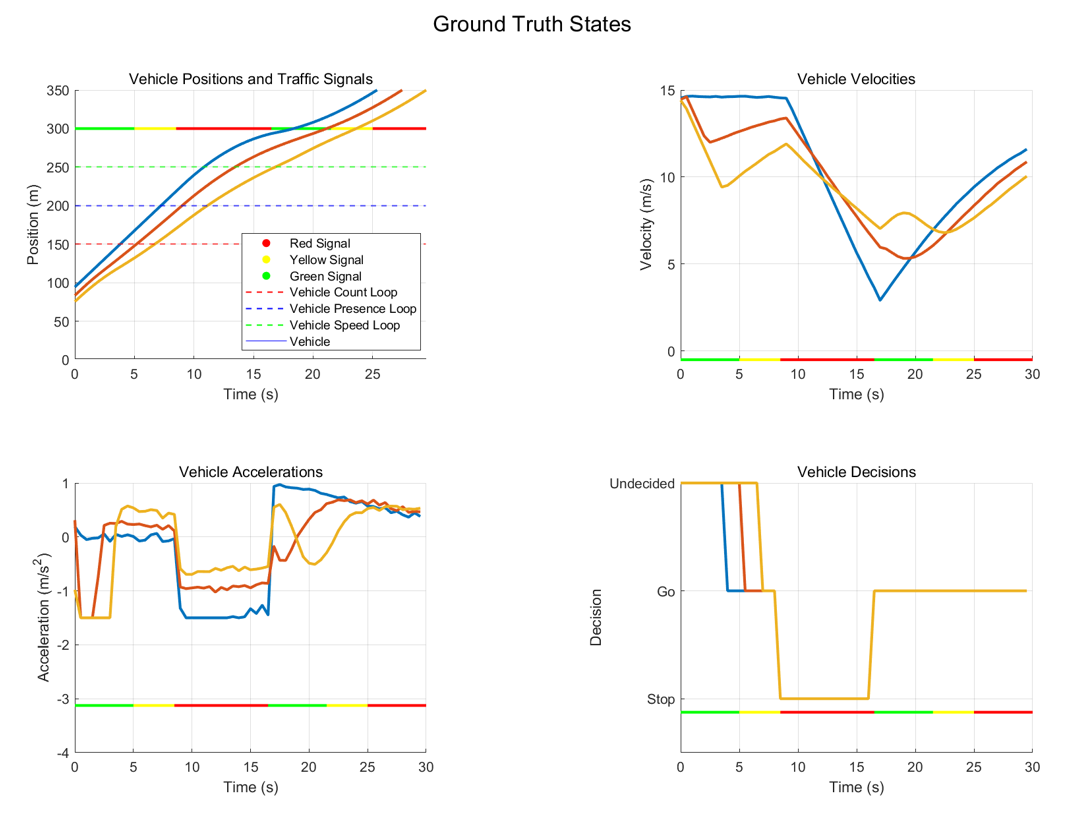
\includegraphics[width= 1\linewidth]{figures/groundtruth-3vehicles.png}
    \caption{Ground truth states, 3vehicles}
    \label{fig: groundtruth-3vehicles}
\end{figure}

In subplot 4, the blue line represents the leading vehicle, showing that it begins making a decision at 4 seconds. In subplot 1, around 4 seconds, the vehicle enters the decision zone and initiates its decision-making process. The parameter $D_h = 150\,\text{m}$ indicates that the vehicle starts making decisions when it approaches 150 meters from the stop line.

The traffic signal timing is as follows: green time is 5 seconds, yellow time is 3.5 seconds, and red time is 8 seconds, with the stop line located at 300 meters. In subplot 1, the vehicle count loop is positioned at 150 meters, the vehicle presence loop at 200 meters, and the vehicle speed loop at 250 meters. In this figure, the leading vehicle decides to stop at the end of the yellow phase and maintains this decision throughout the red phase.


\begin{figure}[H]
    \centering
    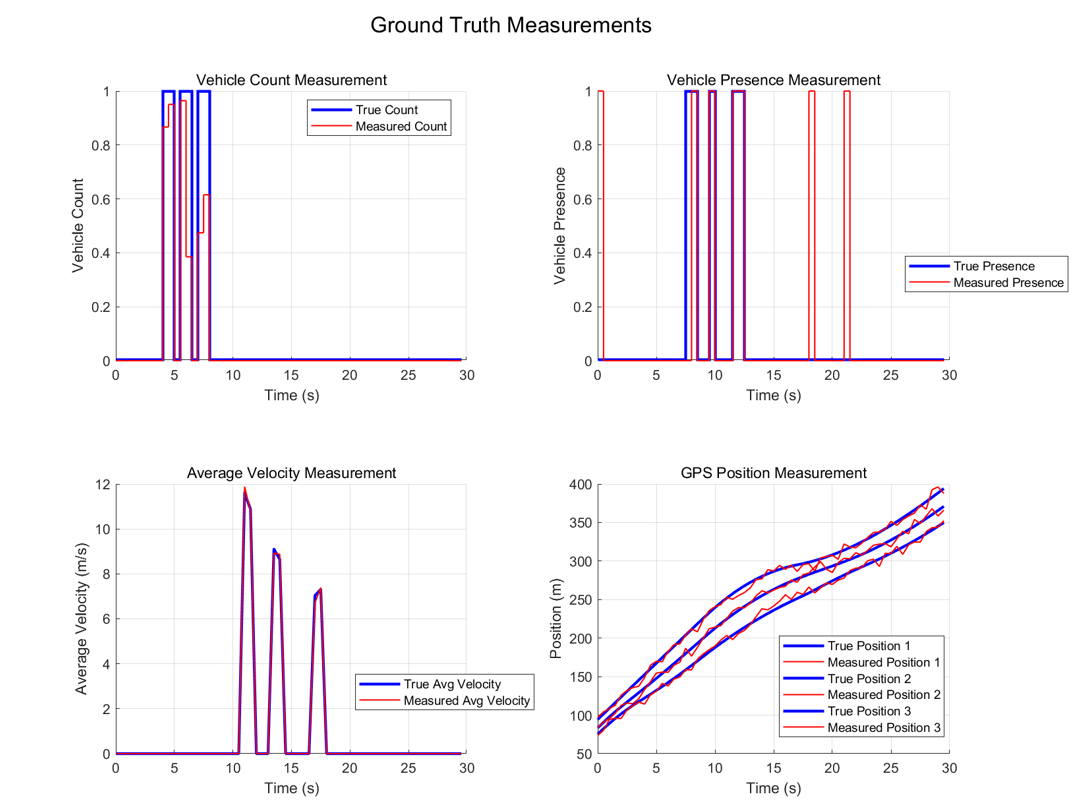
\includegraphics[width= 1\linewidth]{figures/groundtruth measurement.png}
    \caption{Ground truth measurements}
    \label{fig: Ground truth measurements}
\end{figure}

Subplot 1 displays the vehicle count loop, with the true counts occurring around 4, 5.25, and 7 seconds, which aligns with the ground truth states. The measured counts, represented by the red line, are noisy. Subplot 2 shows the vehicle presence loop, where the measured presence aligns with the accuracy parameter of 0.95. Subplot 4 presents the noisy position measurements obtained from GPS. These noisy measurements are intended to serve as inputs for the particle filter during the measurement-based correction step. However, since the particle filter process is not yet complete, these are the full set of simulation results from my work at this stage.

\begin{figure}[H]
    \centering
    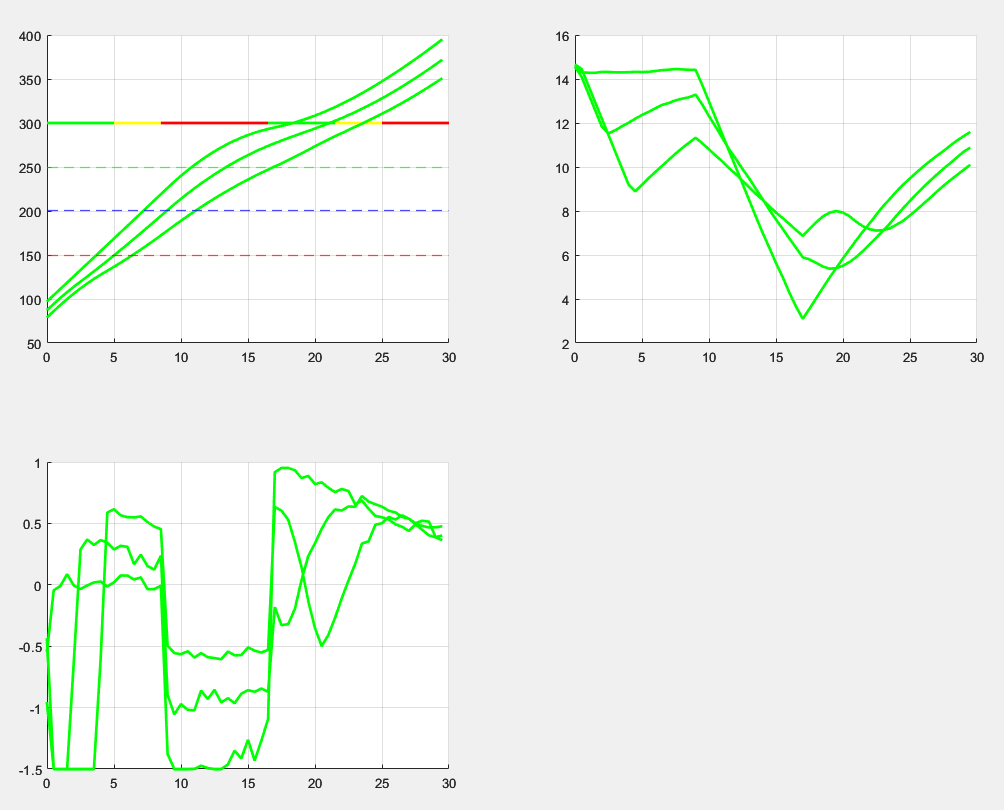
\includegraphics[width= 1\linewidth]{figures/particle filter.png}
    \caption{Unfinished particle filter}
    \label{fig: particle filter}
\end{figure}

The expected outcome is that the green line represents the ground truth states, with particles scattered around it. When the particle filter receives noisy measurements from the loops, particles closer to the ground truth are expected to have larger weights, shows a larger size, reflecting their higher likelihood of accuracy.

\subsection{Procedure}
The procedure will outline the steps for setting initial conditions, starting simulations, and collecting data.
\begin{itemize}
    \item \textbf{Initialization:} To ensure consistency within the particle filter process, the initialization for generating ground truth states, state-based prediction output, and measurement-based correction output follows the same procedure. The initialization step uses predefined bounds to generate initial states for position, velocity, acceleration, and decision for each particle, with each particle representing the states of all vehicles.
    \item \textbf{Simulation:} The simulation begins by generating traffic signal states through the state transition function module. The initial states are then passed to the simulation function to generate the ground truth states and corresponding measurements.
    \item \textbf{Main Process:} In the main script, the ground truth data is plotted, and the initial particles proceed with the state-based prediction. Once the ground truth measurements are received, the particle filter updates the weights, performs resampling, and ultimately produces the state estimations.
\end{itemize}

\subsubsection{Repetitions and Variations}
The parameter \textit{num\_iterations} is adjustable and depends on the traffic signal cycle time. To capture the decision-making process during the yellow phase, \textit{num\_iterations} must be at least longer than the duration of one complete traffic signal cycle.




\subsubsection{Invalidate results: generate state-based prediction output for single vehicle}

\begin{figure}[H]
    \centering
    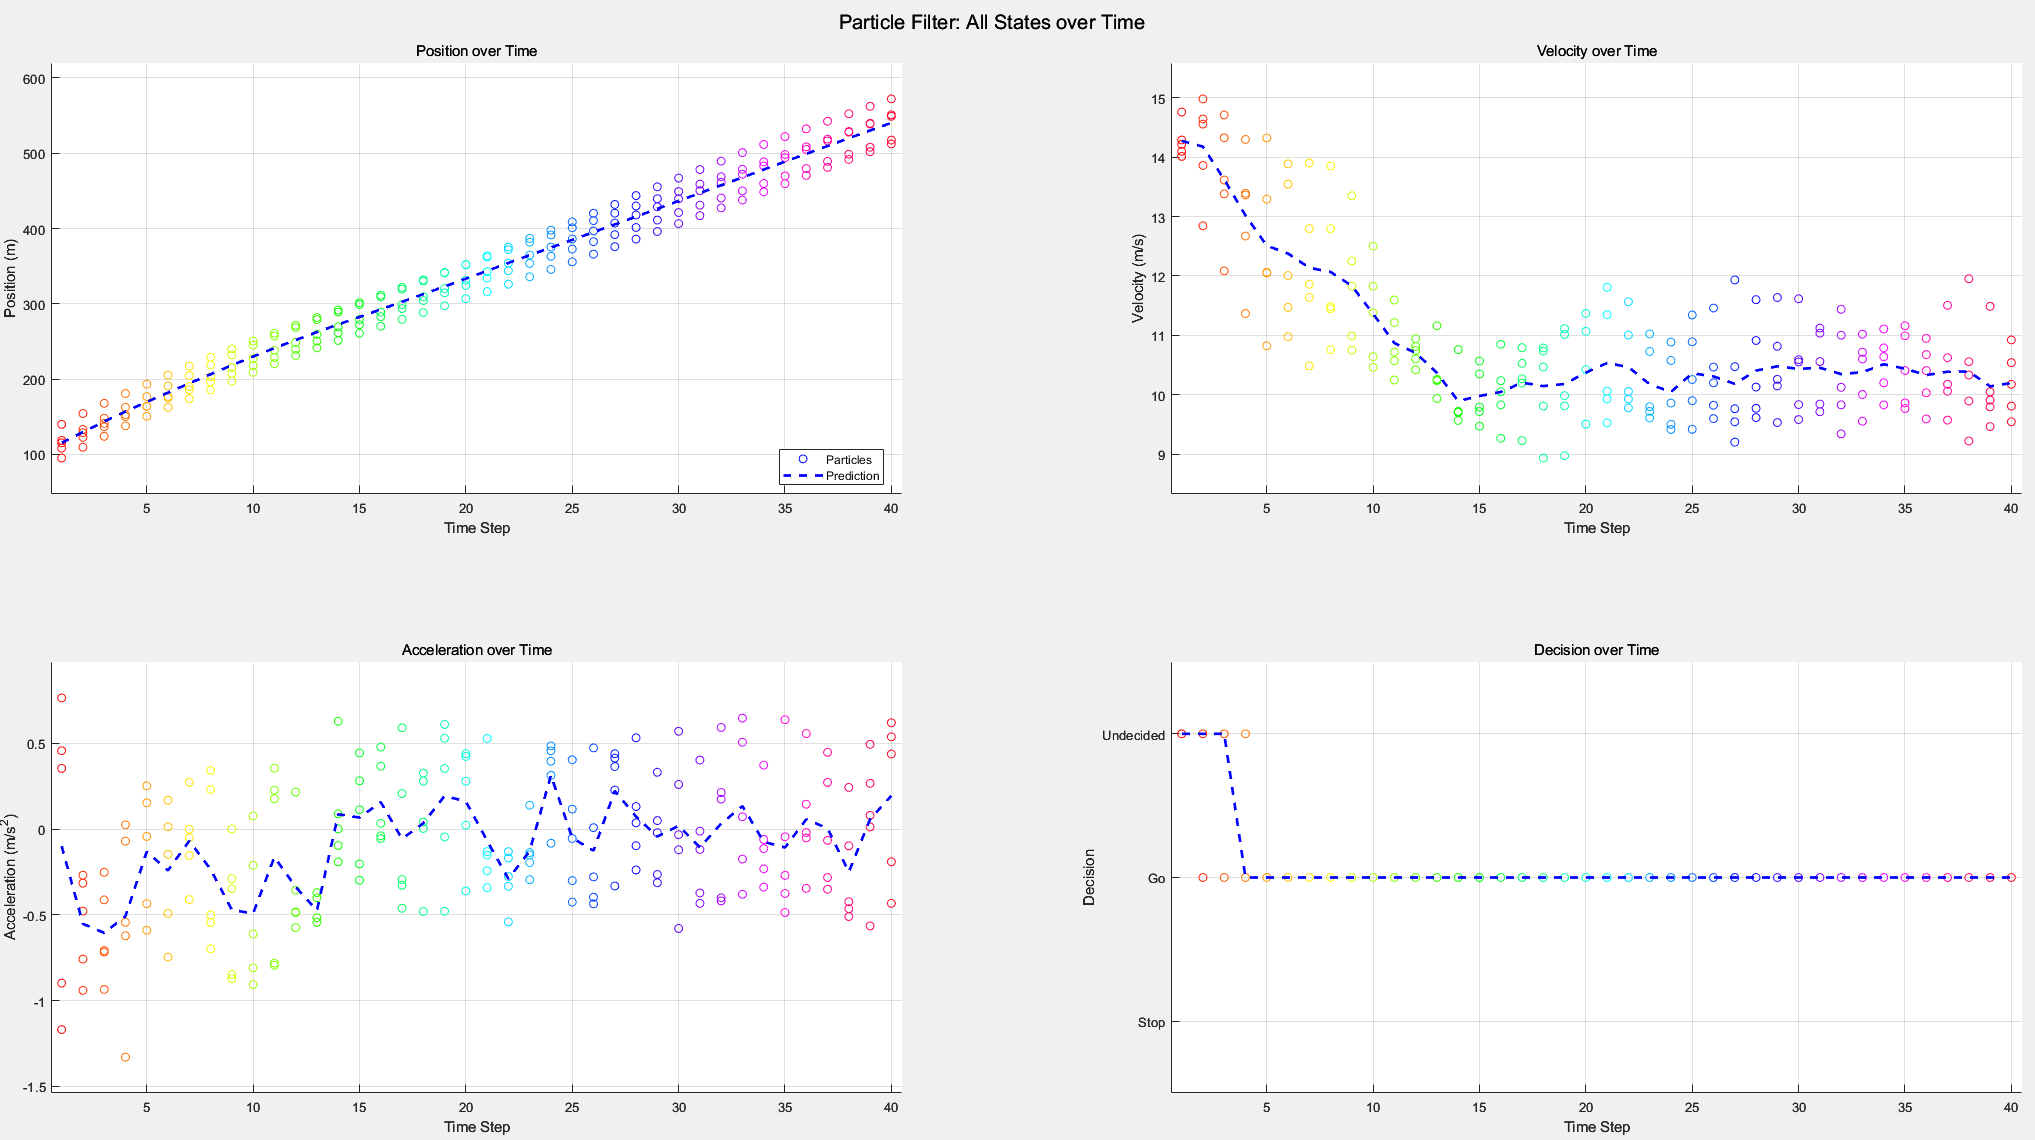
\includegraphics[width= 1\linewidth]{figures/Scenario 1.2.1-1, generate state-based prediction output for single vehicle.png}
    \caption{generate state-based prediction output for single vehicle, $N_\text{particles} = 5$}
    \label{fig: Scenario 1.2.1-1, generate state-based prediction output for single vehicle}
\end{figure}

\begin{figure}[H]
    \centering
    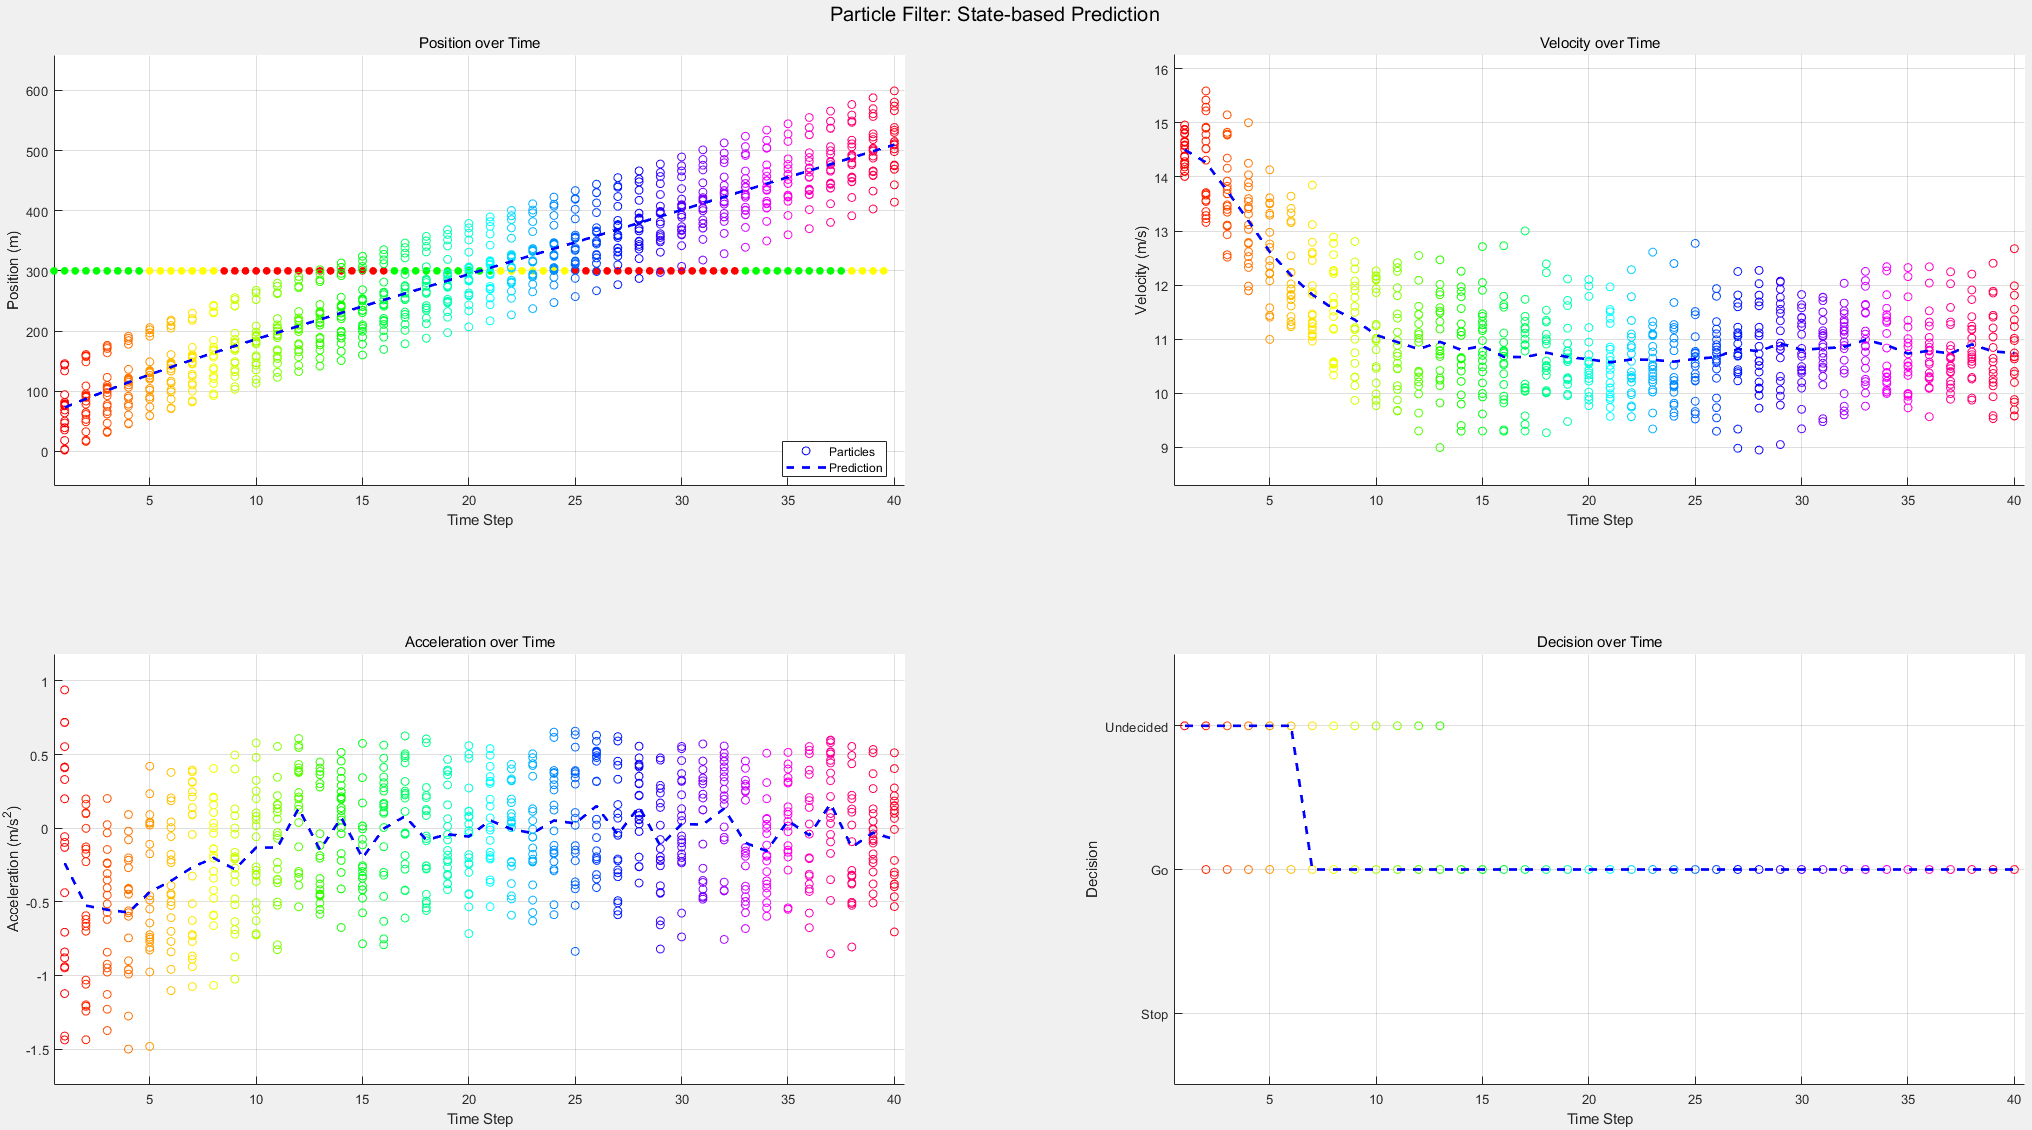
\includegraphics[width= 1\linewidth]{figures/Scenario 1.2.1-2, generate state-based prediction output for single vehicle.png}
    \caption{generate state-based prediction output for single vehicle, $N_\text{particles} = 20$}
    \label{fig: Scenario 1.2.1-2, generate state-based prediction output for single vehicle}
\end{figure}

\begin{figure}[H]
    \centering
    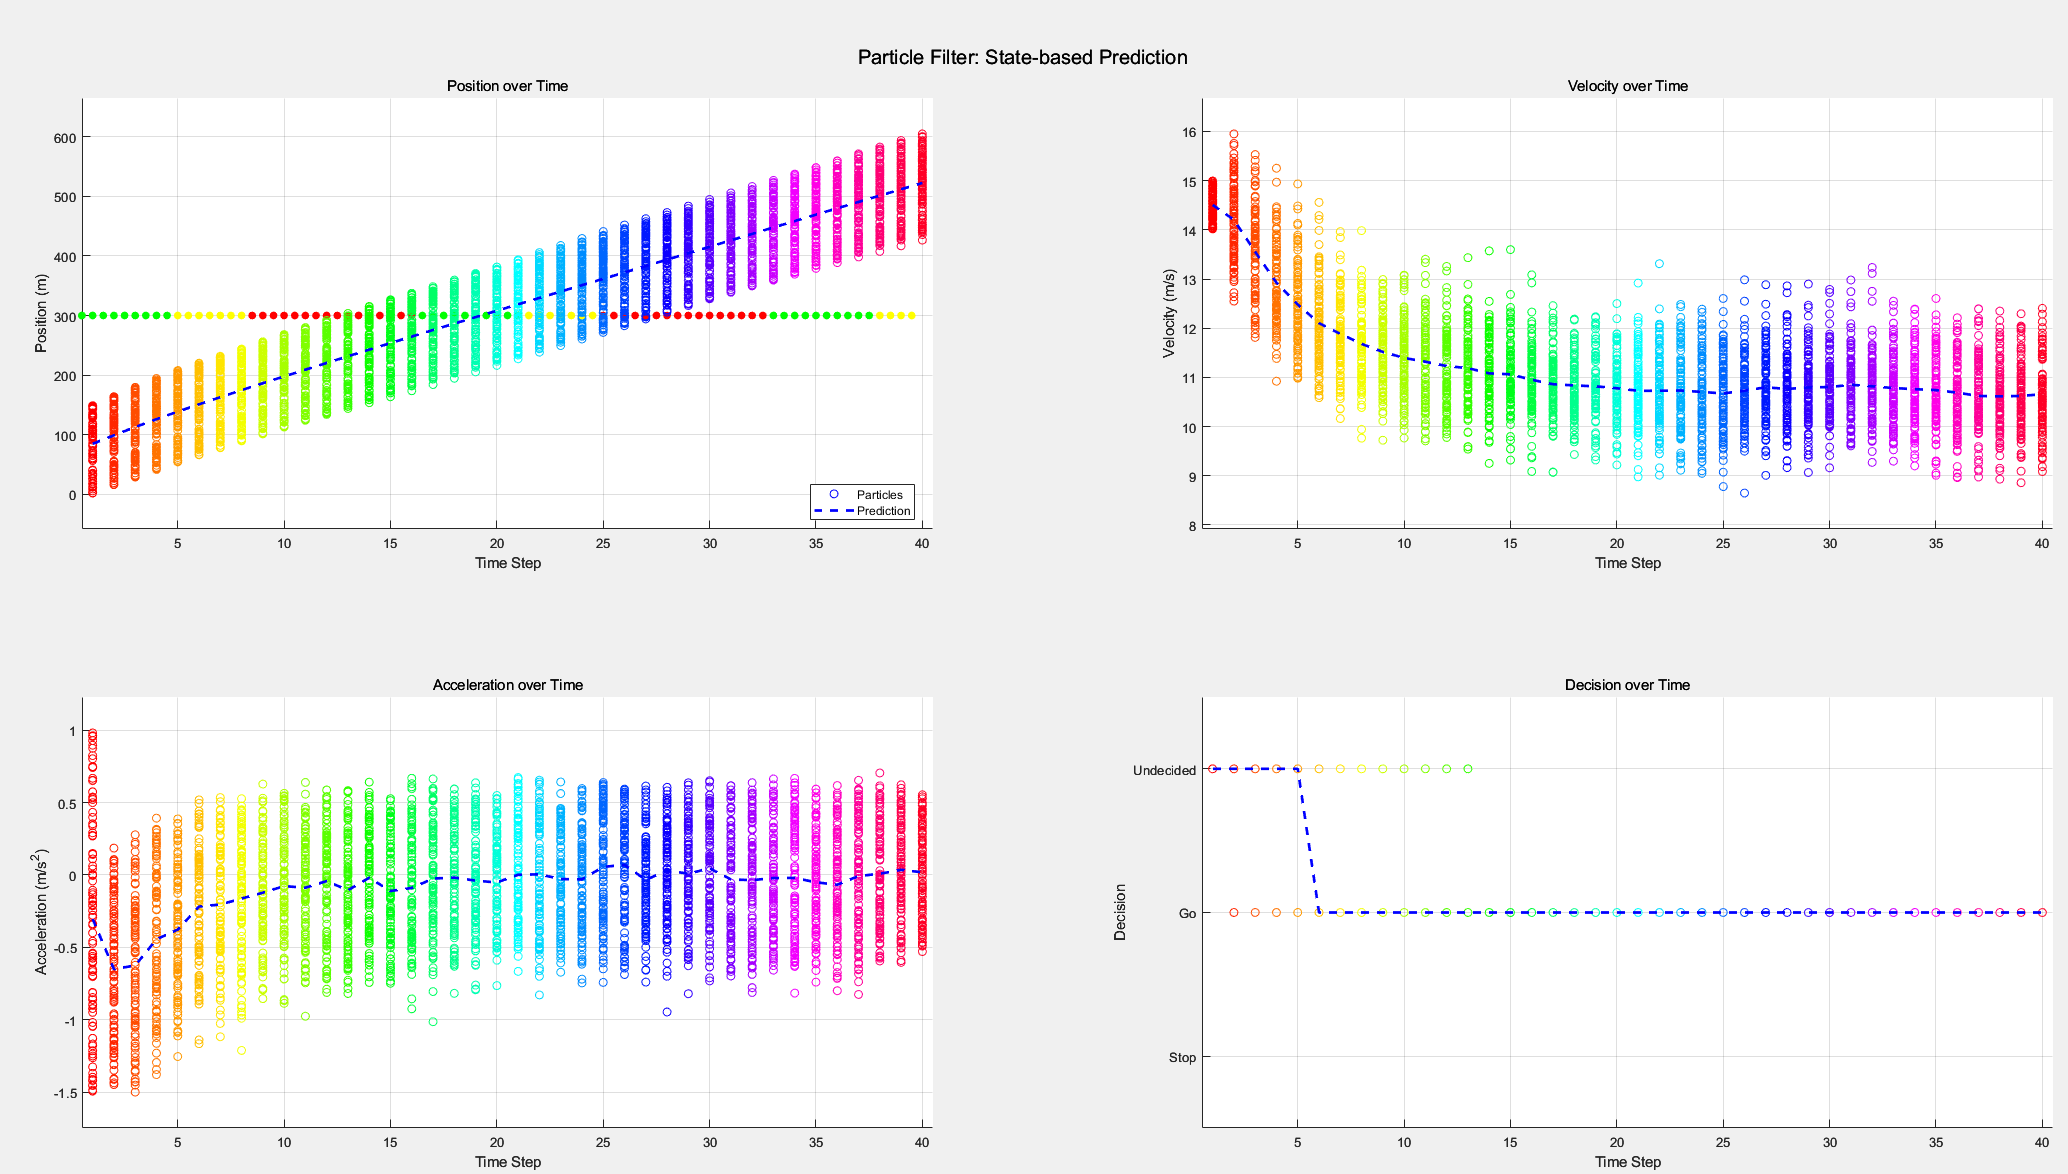
\includegraphics[width= 1\linewidth]{figures/Scenario 1.2.1-3, generate state-based prediction output for single vehicle.png}
    \caption{generate state-based prediction output for single vehicle, $N_\text{particles} = 100$}
    \label{fig: Scenario 1.2.1-3, generate state-based prediction output for single vehicle}
\end{figure}


\subsection{Future Work}
\begin{enumerate}
    \item \textbf{Sensitivity Analysis of $p_\text{stop}$:} \\
    Perform a sensitivity analysis on the decision parameters, particularly $p_\text{stop}$. This involves adjusting these parameters to assess their sensitivity and evaluate their impact on the performance of the PF-SIQE.
    
    \item \textbf{Sensitivity Analysis of Loop Detector Placement:} \\
    Investigate the sensitivity of PF-SIQE to the placement of loop detectors. This entails evaluating whether the performance of the estimator is influenced by the detector locations and, if so, determining the optimal positioning for maximum effectiveness.
    
    \item \textbf{Sensitivity to GPS Penetration Rate:} \\
    Assess the sensitivity of PF-SIQE to the penetration rate of GPS-equipped vehicles. The goal is to identify the minimum proportion of GPS-equipped vehicles required to ensure satisfactory performance of the queue estimator.
    
    \item \textbf{Evaluation of Particle Filter Parameters:} \\
    Explore the influence of particle filter parameters on the performance of PF-SIQE. This includes examining the effects of the number of particles, the threshold for the Effective Particle Number, and the impact of initial conditions. Key parameters to be tested include:
    \begin{itemize}
        \item Number of particles
        \item Threshold for Effective Particle Number
        \item Initial conditions
    \end{itemize}
\end{enumerate}







\section{Discussion}

\subsection{Interpretation of Results}
The primary objective of this thesis was to develop and apply the Particle Filter-Based Signalized Intersection Queue Estimator (PF-SIQE) to estimate vehicle queues at signalized intersections. Although the particle filter process was not fully visualized and validated, the validation of the traffic decision-making model was successfully completed. The ground truth states and the traffic signal state transitions were generated as planned, allowing for an initial evaluation of vehicle behavior during decision-making at intersections.

The key result is that the traffic decision-making model correctly captures vehicle responses in the dilemma zone based on the defined probability ($p_\text{stop}$). These results align with the expected decision patterns of vehicles in real-world scenarios, particularly in the transition from yellow to red lights. However, without the complete execution of the particle filter process, the accuracy of queue estimation and the filter's performance under noisy measurement conditions remain unverified.

\subsection{Validation}
The validation of the traffic decision-making model confirms its effectiveness in representing vehicle behavior in the dilemma zone. The model’s ability to handle stochastic decision-making offers promising potential for future research and application in traffic management systems. However, the particle filter’s validation, which was intended to assess how well the filter handles noisy measurements and updates particle weights, could not be completed due to the visualization challenges. Without this, the core performance of PF-SIQE in accurately estimating queue lengths cannot be fully evaluated at this stage.

\subsection{Limitations}
A significant limitation in this work is the incomplete execution of the particle filter process, which halted the full validation of the PF-SIQE model. As a result, key aspects such as parameter tuning for sensitivity analysis and performance validation under noisy conditions were not conducted. Additionally, due to the absence of real-world data, the model’s validation remains purely simulation-based, and further experiments are needed to verify its effectiveness in real-world applications. Future work should focus on resolving the particle filter visualization issues and extending the validation to include the entire filter process and a broader range of scenarios.

\section{Conclusion}

\subsection{Summary of Findings}
This thesis explored the development of the Particle Filter-Based Signalized Intersection Queue Estimator (PF-SIQE), focusing on real-time queue estimation at signalized intersections. While the particle filter process and its visualization remain incomplete, the traffic decision-making model was successfully validated, showing that it can accurately represent vehicle behavior in the dilemma zone. Ground truth states and measurements were generated as expected, but without completing the particle filter, further results, including accurate queue length estimations, could not be achieved.

\subsection{Implications}
The validation of the traffic decision-making model provides important insights into the potential for applying decision models in traffic management systems. However, the incomplete validation of the PF-SIQE model highlights the need for additional research to fully unlock the estimator's capabilities. Once fully developed and validated, PF-SIQE could significantly improve real-time traffic signal control and optimization by providing accurate queue length estimates, thus contributing to more efficient and adaptive intelligent transportation systems.

\subsection{Future Work}
Future research should focus on completing the particle filter visualization and validation. Key areas for improvement include optimizing the particle filter’s handling of noisy measurements, conducting parameter sensitivity tests, and validating the entire model with real-world traffic data. Expanding the model to incorporate lateral vehicle behavior, lane changes, and multi-lane intersections would also enhance its applicability in more complex urban traffic scenarios. Additionally, extending the research to investigate different particle filter resampling methods and noise models could further improve the accuracy and robustness of the queue estimation process.




